\documentclass[9pt]{beamer}
\usepackage{textpos}
\usepackage{gitinfo2}
\usepackage{csvsimple}
\usepackage{array,booktabs}
\usepackage{url}
\edef\masterBranch{\detokenize{master}}
\edef\gitBranch{\gitBranch}
\setbeamerfont{frametitle}{size=\large}

%fix pandoc's tightlist:https://tex.stackexchange.com/questions/257418/error-tightlist-converting-md-file-into-pdf-using-pandoc#258486
\providecommand{\tightlist}{}%
%  \setlength{\itemsep}{0pt}\setlength{\parskip}{0pt}}

% \usepackage{beamerthemesplit} // Activate for custom appearance

% \usepackage{beamerthemesplit} // Activate for custom appearance

\title{ Spacecraft Requirements, text and rationales
  \tiny{Revision: \gitDescribe, Branch: \gitBranch\\
    For access to the github repository contact edouglas@mit.edu.}}
\author{Authors}
\date{\today}

\begin{document}

%\addtobeamertemplate{frametitle}{}{
%\begin{textblock*}{200mm}(.55\textwidth,-.5cm)
%\includegraphics[height=0.6cm]{bannerlogo.png}
%\end{textblock*}}




\frame{\titlepage}

\section[Outline]{}
\frame{Table of Contents:
\tableofcontents}


\section{Requirement Flow}
\begin{frame}[shrink]{Requirement Flow}
\begin{figure}[htbp]
\begin{center}
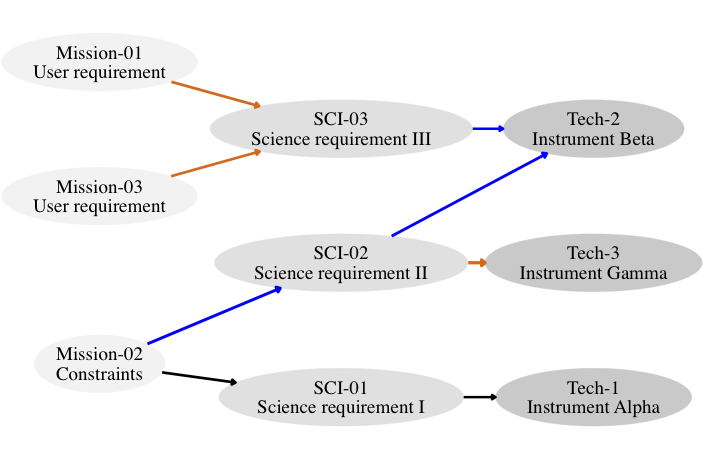
\includegraphics[width=\textwidth]{../Digraph_gv.png}
\label{default}
\end{center}
\end{figure}
\end{frame}

\section{Level 1}
\input{L1_beamer.tex}
\section{Level 2}
\input{L2_beamer.tex}
\section{Level 3}
\input{L3_beamer.tex}


\end{document}
